Diante das limitações identificadas, três abordagens foram consideradas para
expandir a capacidade de instrumentação do veículo: cabeamento dedicado, sistemas
de aquisição independentes e uma ponte sem fio integrada ao fluxo CAN existente.
A literatura sobre sensores sem fio em veículos destaca justamente a redução de
cabeamento, massa e custo de instalação como motivações recorrentes, embora a
confiabilidade do enlace passe a ser uma restrição central de projeto
\cite{tavares2008_wsn_automobiles,rahman2017_intravehicular_wsn,hashemi2014_intracar_multihop_wsn}.

A primeira alternativa seria manter a arquitetura completamente cabeada, usando
acopladores rotativos, chicotes dedicados ou extensões do chicote principal para
alcançar novos pontos de medição. Essa solução preservaria a confiabilidade
física do enlace e exigiria pouco desenvolvimento adicional de \emph{software},
mas deslocaria o problema para a integração mecânica: mais massa, conectores,
proteção, esforço de instalação e menor liberdade para sensores externos ao
veículo ou mudanças rápidas de instrumentação.

A segunda alternativa seria usar módulos autônomos, com aquisição local e memória
própria, recuperados após cada sessão de testes. Embora isso reduza chicotes
longos até o registrador central, a solução rompe a integração com o fluxo de
aquisição em tempo real e exige sincronização posterior dos dados. Além disso,
cada módulo ainda precisa de bateria, condicionamento de sinal e proteção
mecânica, de modo que a massa não desaparece; ela apenas passa a ficar
concentrada no ponto instrumentado.

A alternativa adotada, portanto, é uma ponte de comunicação sem fio entre os
pontos de medição e o sistema de aquisição existente, conforme esquematizado na
Figura~\ref{fig:wcan-semfio}. Nessa abordagem, um nó sensor captura os dados
localmente e os transmite por rádio para um nó receptor conectado ao barramento
CAN do veículo. O receptor injeta os dados na rede como se fossem provenientes
de qualquer outro nó cabeado, tornando a comunicação sem fio transparente para o
restante do sistema. A escolha reduz a dependência de cabos longos e acopladores
rotativos sem abandonar o fluxo de aquisição baseado em identificadores CAN;
ela não elimina os desafios de bateria, encapsulamento, massa localizada e
confiabilidade do enlace sem fio, mas concentra esses desafios em uma solução
compatível com a arquitetura já usada pela equipe. Trabalhos de telemetria em
Fórmula SAE mostram soluções semelhantes, integrando aquisição de dados e
comunicação por rádio com a rede do veículo
\cite{zanetti2013_formula_sae_wireless,visconti2019_formula_sae_telemetry,fernandes2022_formula_sae_wifi_can}.

\begin{figure}[htbp]
\centering
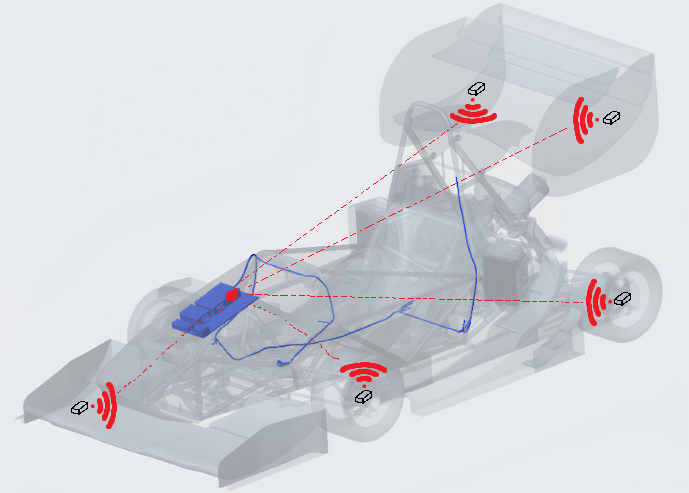
\includegraphics[width=0.65\textwidth]{images/wcan}
\caption{Arquitetura da solução sem fio proposta (WCAN) com transmissão via rádio para receptor central.}
\label{fig:wcan-semfio}
\end{figure}
